Conforme dito anteriormente o trabalho busca o desenvolvimento do design do circuito integrado de um DPD, a partir de um modelo validado em software, e em hardware, no caso, FPGA. Para isso esse projeto foi divido em 4 etapas principais:

\begin{itemize}
    \item Estudo DPD;
    \item Implementação em software;
    \item Implementação em FPGA;
    \item Design e validação do circuito integrado.
\end{itemize}

O cronograma para o desenvolvimento dessas atividades esta disponivel na tabela \ref{tab:cronograma} a seguir:

\begin{table}[ht!]
    \centering
    \renewcommand{\arraystretch}{0.8} % Diminui a altura das linhas
    \setlength{\tabcolsep}{4pt} % Diminui o espaçamento horizontal das células
    \begin{tabular}{|l|c|c|c|c|c|c|c|c|c|}
    \hline
    & mar/24 & abr/24 & mai/24 & jun/24 & jul/24 & ago/24 & set/24 & out/24 & nov/24\\
    \hline
    Etapa 1 & \cellcolor{yellow} & \cellcolor{yellow} &&&&&&& \\
    \rowcolor{gray!20} % Cor da linha
    Etapa 2 && \cellcolor{yellow} & \cellcolor{yellow} & \cellcolor{yellow} &&&&&\\
    Etapa 3 &&& \cellcolor{yellow} & \cellcolor{yellow} & \cellcolor{yellow} & \cellcolor{yellow} &&&\\ 
    \rowcolor{gray!20} % Cor da linha
    Etapa 4 &&&&&& \cellcolor{yellow}& \cellcolor{yellow} & \cellcolor{yellow} & \cellcolor{yellow}\\ 
    \hline
\end{tabular}
\caption{Cronograma de Etapas}
\label{tab:cronograma}
\end{table}
    

\section{Estudo dos DPDs}
A etapa consistiu no estudo dos DPDs, conforme apresentado no Capítulo \ref{chap:revi}, onde foi feito todo o levantamento sobre os tipos de modelagem dos DPDs. O objetivo deste estudo é entender as diferentes abordagens de modelagem, avaliar seus desempenhos e identificar as mais adequadas para a aplicação em amplificadores de potência.

\section{Implementação em software}

Nesta etapa, foi realizada a implementação do modelo DPD em software, utilizando a linguagem de programação Python. Python é uma linguagem amigável, amplamente difundida na comunidade acadêmica e prática de usar.

Para essa modelagem, foram coletados sinais de entrada e saída de um amplificador de potência classe AB, que utiliza um HEMT fabricado com tecnologia GaN. O amplificador foi excitado por um sinal portador de frequência de 900 MHz, modulado por um sinal de envelope WCDMA 3GPP com aproximadamente 3,84 MHz de largura de banda. Os dados de entrada e saída do amplificador de potência foram medidos usando um VSA Rohde \& Schwarz FSQ com uma taxa de amostragem de 61,44 MHz, conforme disponível em \cite{Bonfim2016}.

A seguir, foi realizado o cálculo da estimativa do sinal utilizando números com vírgula fixa. Para verificar a precisão dessa estimativa em relação ao sinal original, foi calculado o NMSE. Para essa validação, os dados foram inicialmente divididos em conjuntos de extração e validação. A matriz de confusão\footnote{Uma matriz de confusão em um polinômio de memória é uma ferramenta analítica usada para visualizar e avaliar o desempenho do modelo, comparando as saídas previstas com as saídas reais. A matriz normalmente resume os resultados das previsões em termos de verdadeiros positivos, falsos positivos, verdadeiros negativos e falsos negativos.} foi calculada com os dados de extração, utilizando o código disponível no anexo \ref{cod:mp}. Esse cálculo é essencial para a extração dos coeficientes do polinômio de memória. Após a extração dos coeficientes, foi calculado o modelo do PA, que foi então validado com os dados de validação. O NMSE obtido para um polinômio de 2° grau com uma amostra memorizada foi de -23,57 dB.

Em seguida, o algoritmo foi ajustado para operar com números em vírgula fixa e o número total de bits foi reajustado para atingir a menor resolução possível, buscando o menor NMSE simulado, conforme ilustrado pelo anexo \ref{cod:mpint}. Perceba que por ser tratar de um calculo em virgula fixa, foi necessário fazer uma readequação do resultado obtido entre cada multiplicação de forma a manter a resolução inicial.

\section{Implementação em FPGA}
Essa etapa consiste na implementação do DPD em FPGA. Para isso, é necessário realizar paralelizações nas operações aritméticas. A Figura \ref{fig:diagramaprocess} ilustra como esse processo está dividido entre cada ciclo de clock. A cada ciclo, duas operações ocorrem de forma paralela: a elevação do sinal atual ao quadrado e o registro deste sinal, além do somatório da multiplicação dos sinais do mesmo instante de tempo pelo seu respectivo coeficiente. Esse processo ocorre P vezes para os P graus do polinômio de memória. Portanto, a saída do DPD é inválida para os primeiros P períodos de clock.

\begin{figure}[ht!]
    \centering
    \captionsetup{justification=centering}
    \caption*{Fonte: Autor}
    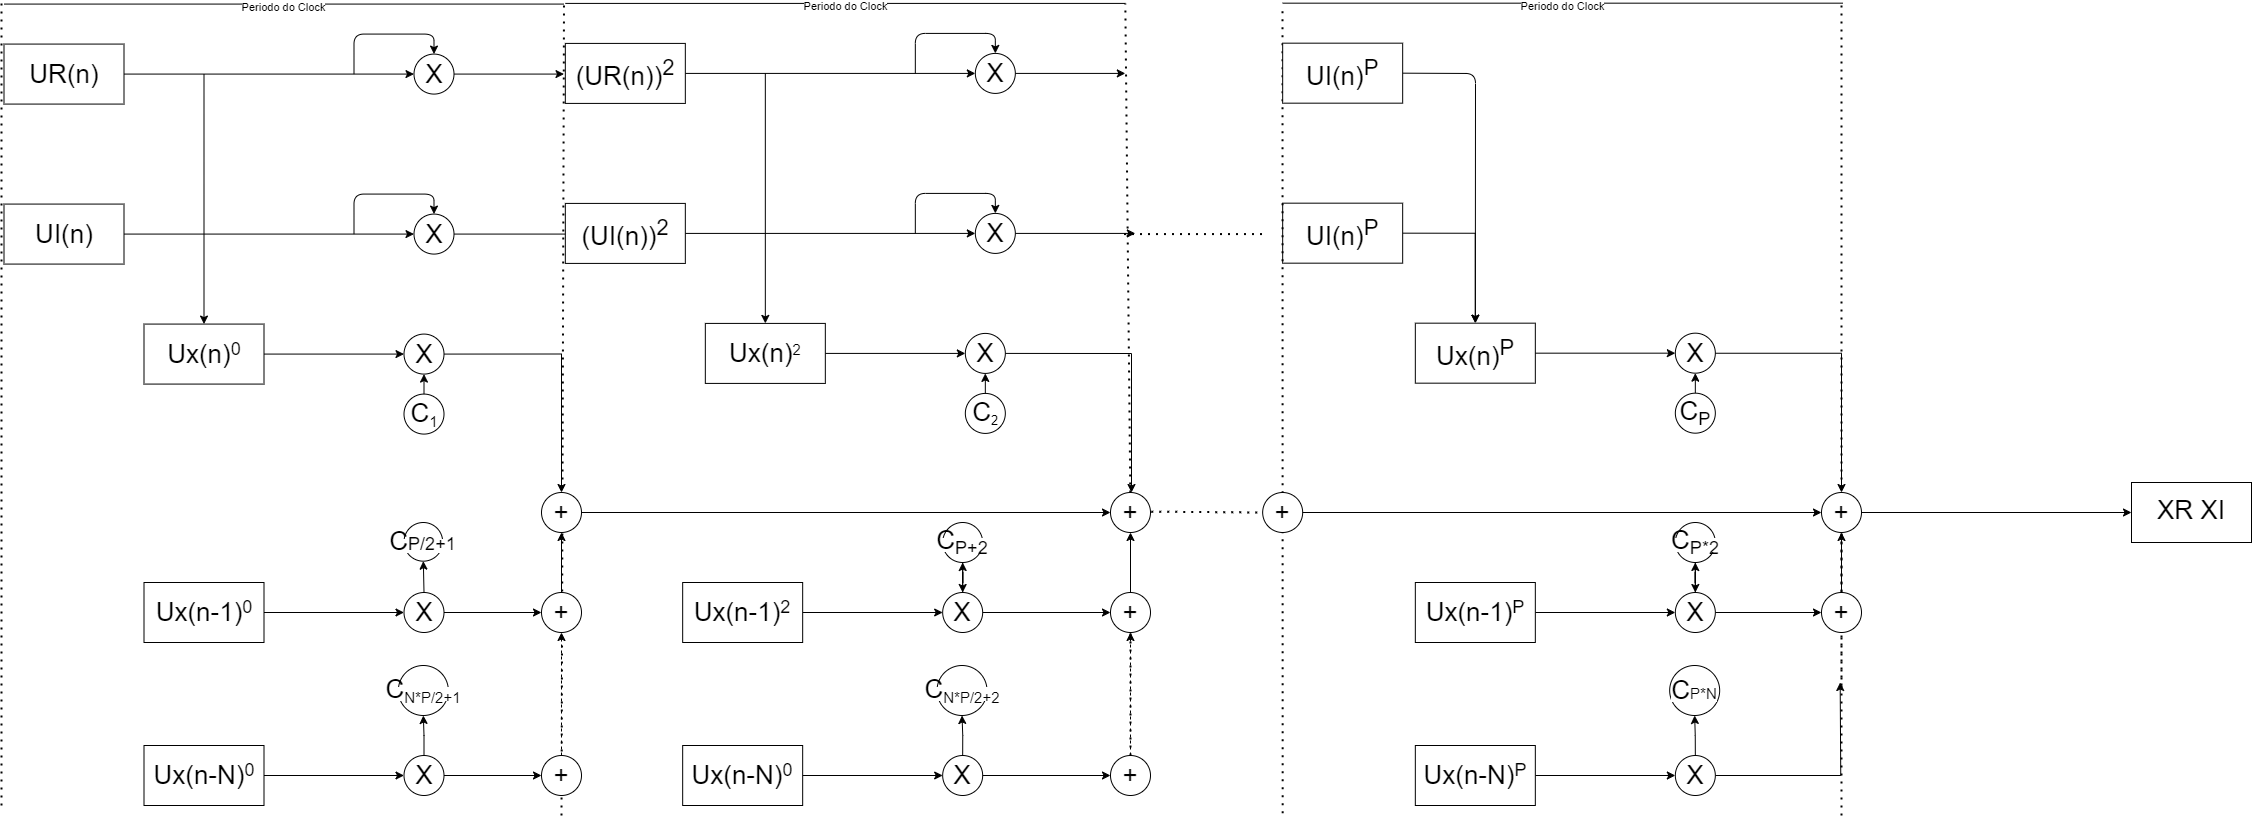
\includegraphics[width=0.5\textwidth]{diagrama_process.png}
    \caption{Processo de calculo da saida}
    \label{fig:diagramaprocess}
\end{figure}

\section{Design e validação}
Finalmente, na última etapa, realiza-se o processo de concepção do circuito integrado do DPD como um circuito dedicado integrado na tecnologia BiCMOS 130 nm 8HP, utilizando as ferramentas do Cadence.
O fluxo de projeto VLSI  para design de um circuito integrado de aplicação específica, inclui a descrição do circuito em VHDL, síntese lógica utilizando as células padrão da tecnologia, place and route e simulações comportamentais e temporais. O diagrama do fluxo VLSI pode ser ilustrado pela figura \ref{fig:CMOS2010}.

\begin{figure}[ht!]
    \centering
    \captionsetup{justification=centering}
    \caption*{Fonte: \cite{CMOS2010}}
    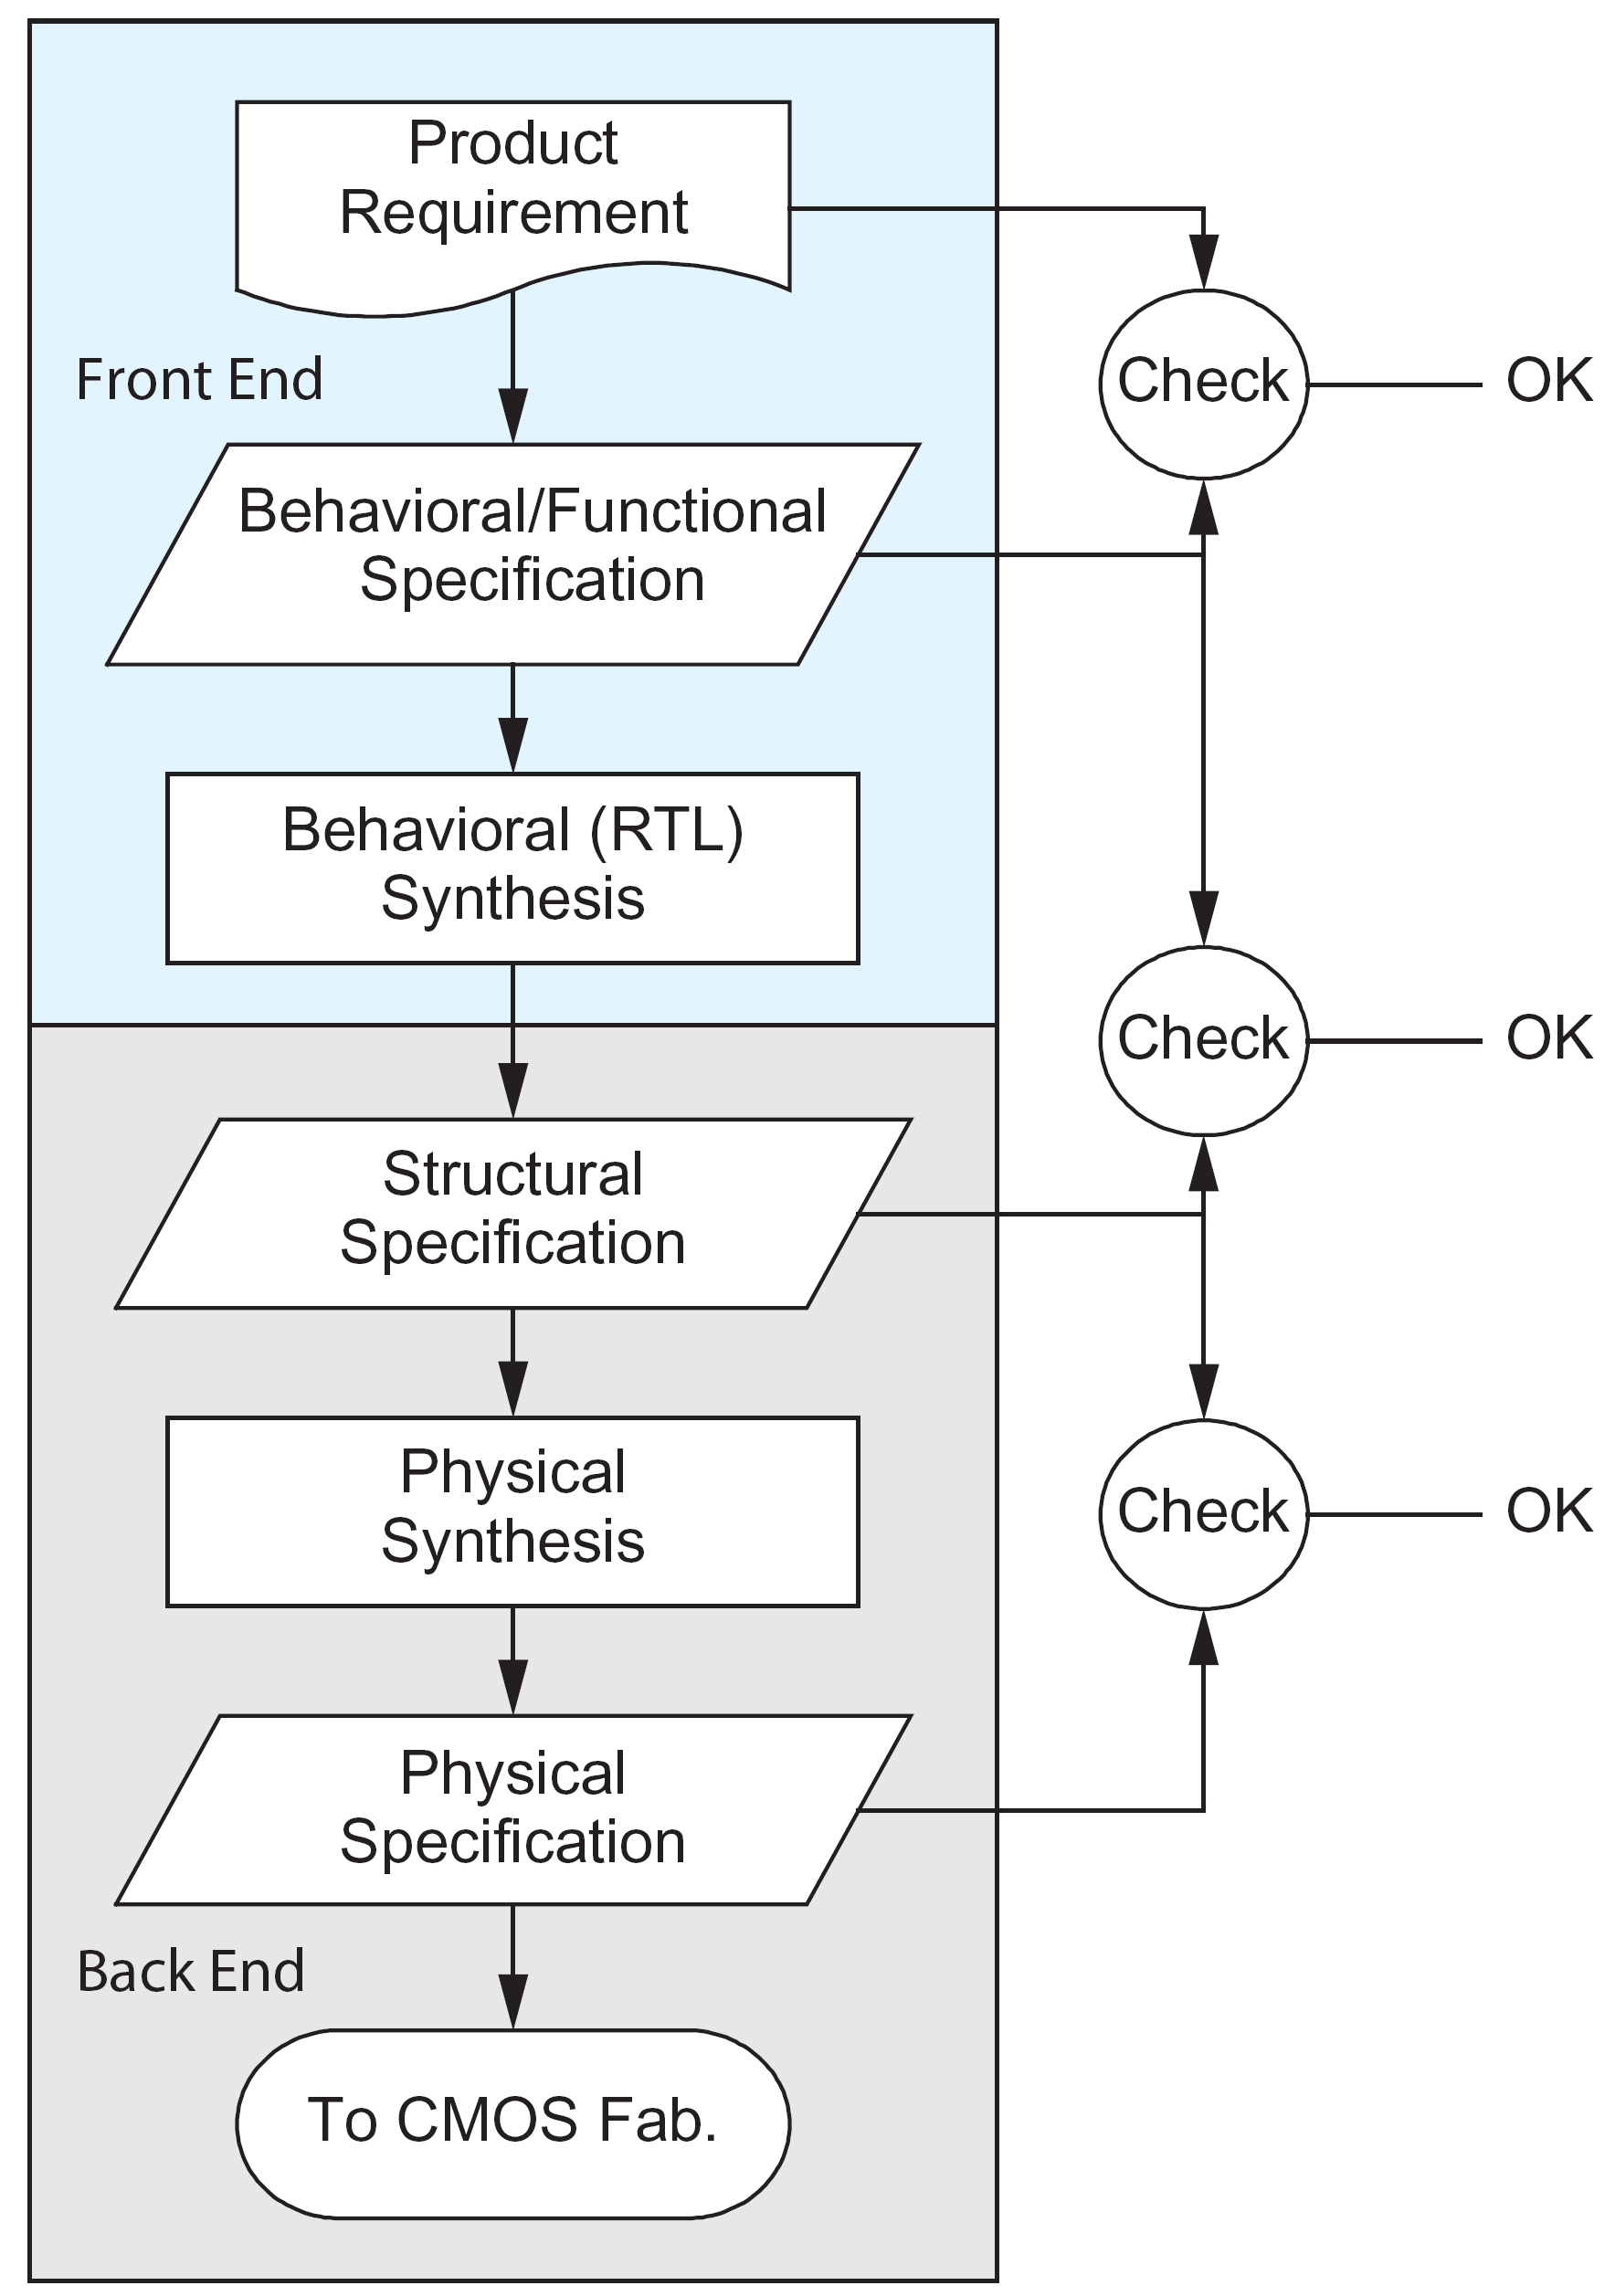
\includegraphics[width=0.5\textwidth]{fluxovlsi.png}
    \caption{Fluxo de projeto VLSI}
    \label{fig:CMOS2010}
\end{figure}

No processo de desenvolvimento do circuito, várias etapas são executadas. Primeiro, há a simulação comportamental para verificar se o circuito VHDL atende às expectativas, utilizando um testbench em VHDL e a ferramenta Cadence NCLaunch. Em seguida, ocorre a síntese lógica, onde a partir do modelo comportamental, utiliza-se a ferramenta Genus para criar um modelo RTL com células padrão de tecnologia específica, considerando restrições de área, frequência e consumo de energia. A síntese gera dois arquivos: um com componentes e conexões, em Verilog, e outro com informações de atraso no formato SDF. A simulação pós-síntese é realizada para validar o netlist gerado, usando o mesmo testbench da simulação comportamental. Em seguida, na etapa de PAR, o layout é criado posicionando as células e realizando as conexões entre essas células, utilizando a ferramenta Innovus. Por fim, na simulação pós-PAR, o circuito é simulado considerando as resistências e capacitâncias parasitas. Cada etapa é fundamental para garantir o correto funcionamento do circuito.

